\documentclass[12pt]{report}

% ---------- Packages ----------
\usepackage[utf8]{inputenc}
\usepackage[T1]{fontenc}
\usepackage[a4paper,margin=1in]{geometry}
\usepackage{array}
\usepackage{graphicx}
\usepackage{float}
\usepackage{caption}
\usepackage{fancyhdr}
\usepackage[colorlinks=true, linkcolor=blue, citecolor=blue, urlcolor=blue]{hyperref}

% ---------- Section numbering: this file is Chapter Two ----------
\renewcommand{\thesection}{2.\arabic{section}}
\renewcommand{\thesubsection}{2.\arabic{section}.\arabic{subsection}}

% ---------- Running header: centred chapter title, rule below ----------
\pagestyle{fancy}
\setlength{\headheight}{15pt}
\fancyhf{}
\fancyhead[C]{\bfseries Chapter Two: Problem Analysis}
\fancyfoot[C]{\thepage}
\renewcommand{\headrulewidth}{0.4pt}
\renewcommand{\footrulewidth}{0pt}

\begin{document}

% ---------- Chapter-opening page ----------
\thispagestyle{empty}
\vspace*{\stretch{1}}
\begin{center}
{\Large\bfseries Chapter Two}\\[1em]
{\Large\bfseries Problem Analysis}
\end{center}
\vspace*{\stretch{2}}
\clearpage

\section{Input Analysis}

The system reads input only from the console keyboard. There is no file input, no network input and no stored configuration. Nine distinct inputs exist across the six menu options.

\begin{enumerate}

\item \textbf{Menu choice}
\begin{itemize}
\item \textbf{Where entered:} main menu
\item \textbf{Data type and size:} unsigned byte
\item \textbf{Valid range:} 1 to 6
\item \textbf{Validation rule:} must be an integer from 1 to 6
\item \textbf{Error response:} show ``Invalid choice'' and redisplay the menu
\end{itemize}

\item \textbf{Customer name}
\begin{itemize}
\item \textbf{Where entered:} Book New Ticket
\item \textbf{Data type and size:} ASCII string, 1 byte per character, stored in a 21-byte field (20 characters plus a null terminator)
\item \textbf{Valid range:} 1--20 characters
\item \textbf{Validation rule:} must not be empty and must not exceed 20 characters
\item \textbf{Error response:} show a name error and re-prompt
\end{itemize}

\item \textbf{Booking ID (new)}
\begin{itemize}
\item \textbf{Where entered:} Book New Ticket
\item \textbf{Data type and size:} unsigned doubleword
\item \textbf{Valid range:} 100000--999999
\item \textbf{Validation rule:} must be exactly six digits in range, and must not match the ID of any \textbf{active} record
\item \textbf{Error response:} out of range, re-prompt; duplicate, ``ERROR: Booking ID already exists!''
\end{itemize}

\item \textbf{Movie code}
\begin{itemize}
\item \textbf{Where entered:} Book New Ticket
\item \textbf{Data type and size:} unsigned byte
\item \textbf{Valid range:} 1 to 3
\item \textbf{Validation rule:} 1 = Movie A, 2 = Movie B, 3 = Movie C
\item \textbf{Error response:} show a movie code error and re-prompt
\end{itemize}

\item \textbf{Seat number}
\begin{itemize}
\item \textbf{Where entered:} Book New Ticket
\item \textbf{Data type and size:} unsigned byte
\item \textbf{Valid range:} 1 to 20
\item \textbf{Validation rule:} must be in range \textbf{and} currently free in the seat map of the chosen movie
\item \textbf{Error response:} out of range, re-prompt; taken, ``ERROR: Seat already reserved!''
\end{itemize}

\item \textbf{Ticket category}
\begin{itemize}
\item \textbf{Where entered:} Book New Ticket
\item \textbf{Data type and size:} unsigned byte
\item \textbf{Valid range:} 1 to 3
\item \textbf{Validation rule:} 1 = Adult, 2 = Student, 3 = Child
\item \textbf{Error response:} show a category error and re-prompt
\end{itemize}

\item \textbf{Booking ID (cancel)}
\begin{itemize}
\item \textbf{Where entered:} Cancel Booking
\item \textbf{Data type and size:} unsigned doubleword
\item \textbf{Valid range:} 100000--999999
\item \textbf{Validation rule:} must match an \textbf{active} record
\item \textbf{Error response:} ``ERROR: Booking ID not found!''
\end{itemize}

\item \textbf{Booking ID (display)}
\begin{itemize}
\item \textbf{Where entered:} Display Ticket
\item \textbf{Data type and size:} unsigned doubleword
\item \textbf{Valid range:} 100000--999999
\item \textbf{Validation rule:} must match an \textbf{active} record
\item \textbf{Error response:} ``ERROR: Booking ID not found!''
\end{itemize}

\item \textbf{Movie code (seat map)}
\begin{itemize}
\item \textbf{Where entered:} Display Seating Map
\item \textbf{Data type and size:} unsigned byte
\item \textbf{Valid range:} 1 to 3
\item \textbf{Validation rule:} 1 to 3 only
\item \textbf{Error response:} show a movie code error and re-prompt
\end{itemize}

\end{enumerate}

\subsection*{Why these data sizes}

The sizes above follow directly from the integer storage sizes studied in Chapter One:

\begin{itemize}
\item A \textbf{byte} stores an unsigned value from \textbf{0 to 255}. This covers the menu choice (1 to 6), the movie code (1 to 3), the seat number (1 to 20), the ticket category (1 to 3) and the active flag (0 or 1) with a large margin, so a byte is the correct and cheapest choice for all five.
\item A \textbf{word} stores an unsigned value from \textbf{0 to 65,535}. This is \textbf{too small for a booking ID}, because the largest legal ID, 999,999, is far beyond 65,535 and would overflow the field.
\item A \textbf{doubleword} stores an unsigned value from \textbf{0 to 4,294,967,295}, which holds any six-digit booking ID comfortably. Prices and revenue totals are also kept in doublewords so that all arithmetic operands share one width.
\item The customer name is stored as \textbf{ASCII characters, one byte per character}, as covered in the character-storage topic of Chapter One. The name field is 21 bytes: 20 character codes plus one byte for the terminating null that marks the end of the string.
\end{itemize}

\subsection*{Stored inputs and transient inputs}

The width of an input is decided by the range of values it must hold, and nothing else. A value is never given a wider field just because it is typed at the keyboard.

Four of the nine inputs are \textbf{stored}: the customer name, the booking ID, the movie code, the seat number and the ticket category are written into a booking record and must stay there for the life of the booking. Their widths add up to the record size, so every byte counts.

The remaining inputs are \textbf{transient}. The menu choice, the booking ID used to cancel or to display a ticket, and the movie code used to pick a seating map are read, checked, acted upon and then discarded. None of them occupies space in a record. Even so, each is sized by its own range: the menu choice and the seat-map movie code fit in a byte, while a transient booking ID still needs a doubleword, because 999,999 overflows a word no matter how briefly the value is held.

\subsection*{Capacity checks before a booking is accepted}

Two further conditions are tested during booking. They are not typed by the user, but a booking is rejected if either fails:

\begin{enumerate}
\item \textbf{System capacity:} the system holds at most \textbf{60 active bookings}. An attempt to create the 61st produces \texttt{"ERROR: Cinema capacity reached!"}.
\item \textbf{Hall capacity:} each movie has \textbf{20 seats}. When all 20 seats of a movie are reserved, that movie is full and no further seat in it can be chosen.
\end{enumerate}

\subsection*{Non-numeric input}

Every numeric prompt (menu choice, booking ID, seat number, movie code, ticket category) checks that the entered characters are digits before any range check runs. A prompt that receives a non-digit character shows the same error as an out-of-range value and re-reads the field, so a stray letter can never reach the range or lookup logic below it.

\section{Output Analysis}

All output is formatted console text. Each output is produced on demand from the data currently held in memory; nothing is written to a file.

\begin{enumerate}

\item \textbf{Main menu}
\begin{itemize}
\item \textbf{Trigger:} program start and after every completed operation
\item \textbf{Format:} banner line, six numbered options, input prompt
\item \textbf{Data source:} fixed text
\end{itemize}

\item \textbf{Input prompts}
\begin{itemize}
\item \textbf{Trigger:} during every operation
\item \textbf{Format:} one short line per field, stating the legal range
\item \textbf{Data source:} fixed text
\end{itemize}

\item \textbf{Booking confirmation}
\begin{itemize}
\item \textbf{Trigger:} a booking is accepted
\item \textbf{Format:} \texttt{Booking added successfully!} followed by \texttt{Final Ticket Price: n JOD}
\item \textbf{Data source:} final price just calculated
\end{itemize}

\item \textbf{Formatted ticket}
\begin{itemize}
\item \textbf{Trigger:} menu option 3 with a valid active ID
\item \textbf{Format:} banner, customer name, booking ID, movie, seat, category, base price, discount, separator line, final price
\item \textbf{Data source:} one active booking record
\end{itemize}

\item \textbf{Seating map}
\begin{itemize}
\item \textbf{Trigger:} menu option 4 with a valid movie code
\item \textbf{Format:} title, legend \texttt{[O] Available [X] Reserved}, 4 rows of 5 seats, reserved count, occupancy percentage
\item \textbf{Data source:} seat map of the selected movie
\end{itemize}

\item \textbf{Per-movie statistics}
\begin{itemize}
\item \textbf{Trigger:} menu option 5
\item \textbf{Format:} one line per movie: bookings, revenue in JOD, occupancy percentage
\item \textbf{Data source:} per-movie counters and revenue totals
\end{itemize}

\item \textbf{Overall totals}
\begin{itemize}
\item \textbf{Trigger:} menu option 5
\item \textbf{Format:} total active bookings, overall revenue, average ticket price
\item \textbf{Data source:} totals accumulated over the active records
\end{itemize}

\item \textbf{Most and least booked movie}
\begin{itemize}
\item \textbf{Trigger:} menu option 5
\item \textbf{Format:} two labelled lines naming one movie each
\item \textbf{Data source:} the three per-movie booking counts
\end{itemize}

\item \textbf{Category histogram}
\begin{itemize}
\item \textbf{Trigger:} menu option 5
\item \textbf{Format:} one row per category, a run of asterisks, and the count in brackets
\item \textbf{Data source:} the three category counters
\end{itemize}

\item \textbf{Error messages}
\begin{itemize}
\item \textbf{Trigger:} any failed validation
\item \textbf{Format:} a single line beginning \texttt{ERROR:} where specified, otherwise a short explanatory line, followed by a re-prompt
\item \textbf{Data source:} fixed text
\end{itemize}

\end{enumerate}

All ten outputs are plain console text produced through \textbf{library calls}, which is the highest of the four input-output levels studied in Chapter Two. The program does not call BIOS routines and does not address hardware ports directly. This is what keeps the program portable across lab machines, and it is the reason graphics, colour control and printer output are excluded from the project scope.

\section{Process Flow}

\subsection{Main program flow}

\begin{minipage}{\textwidth}
The program initialises its data once, then repeats a menu cycle until the user chooses to exit.

\medskip
\centering
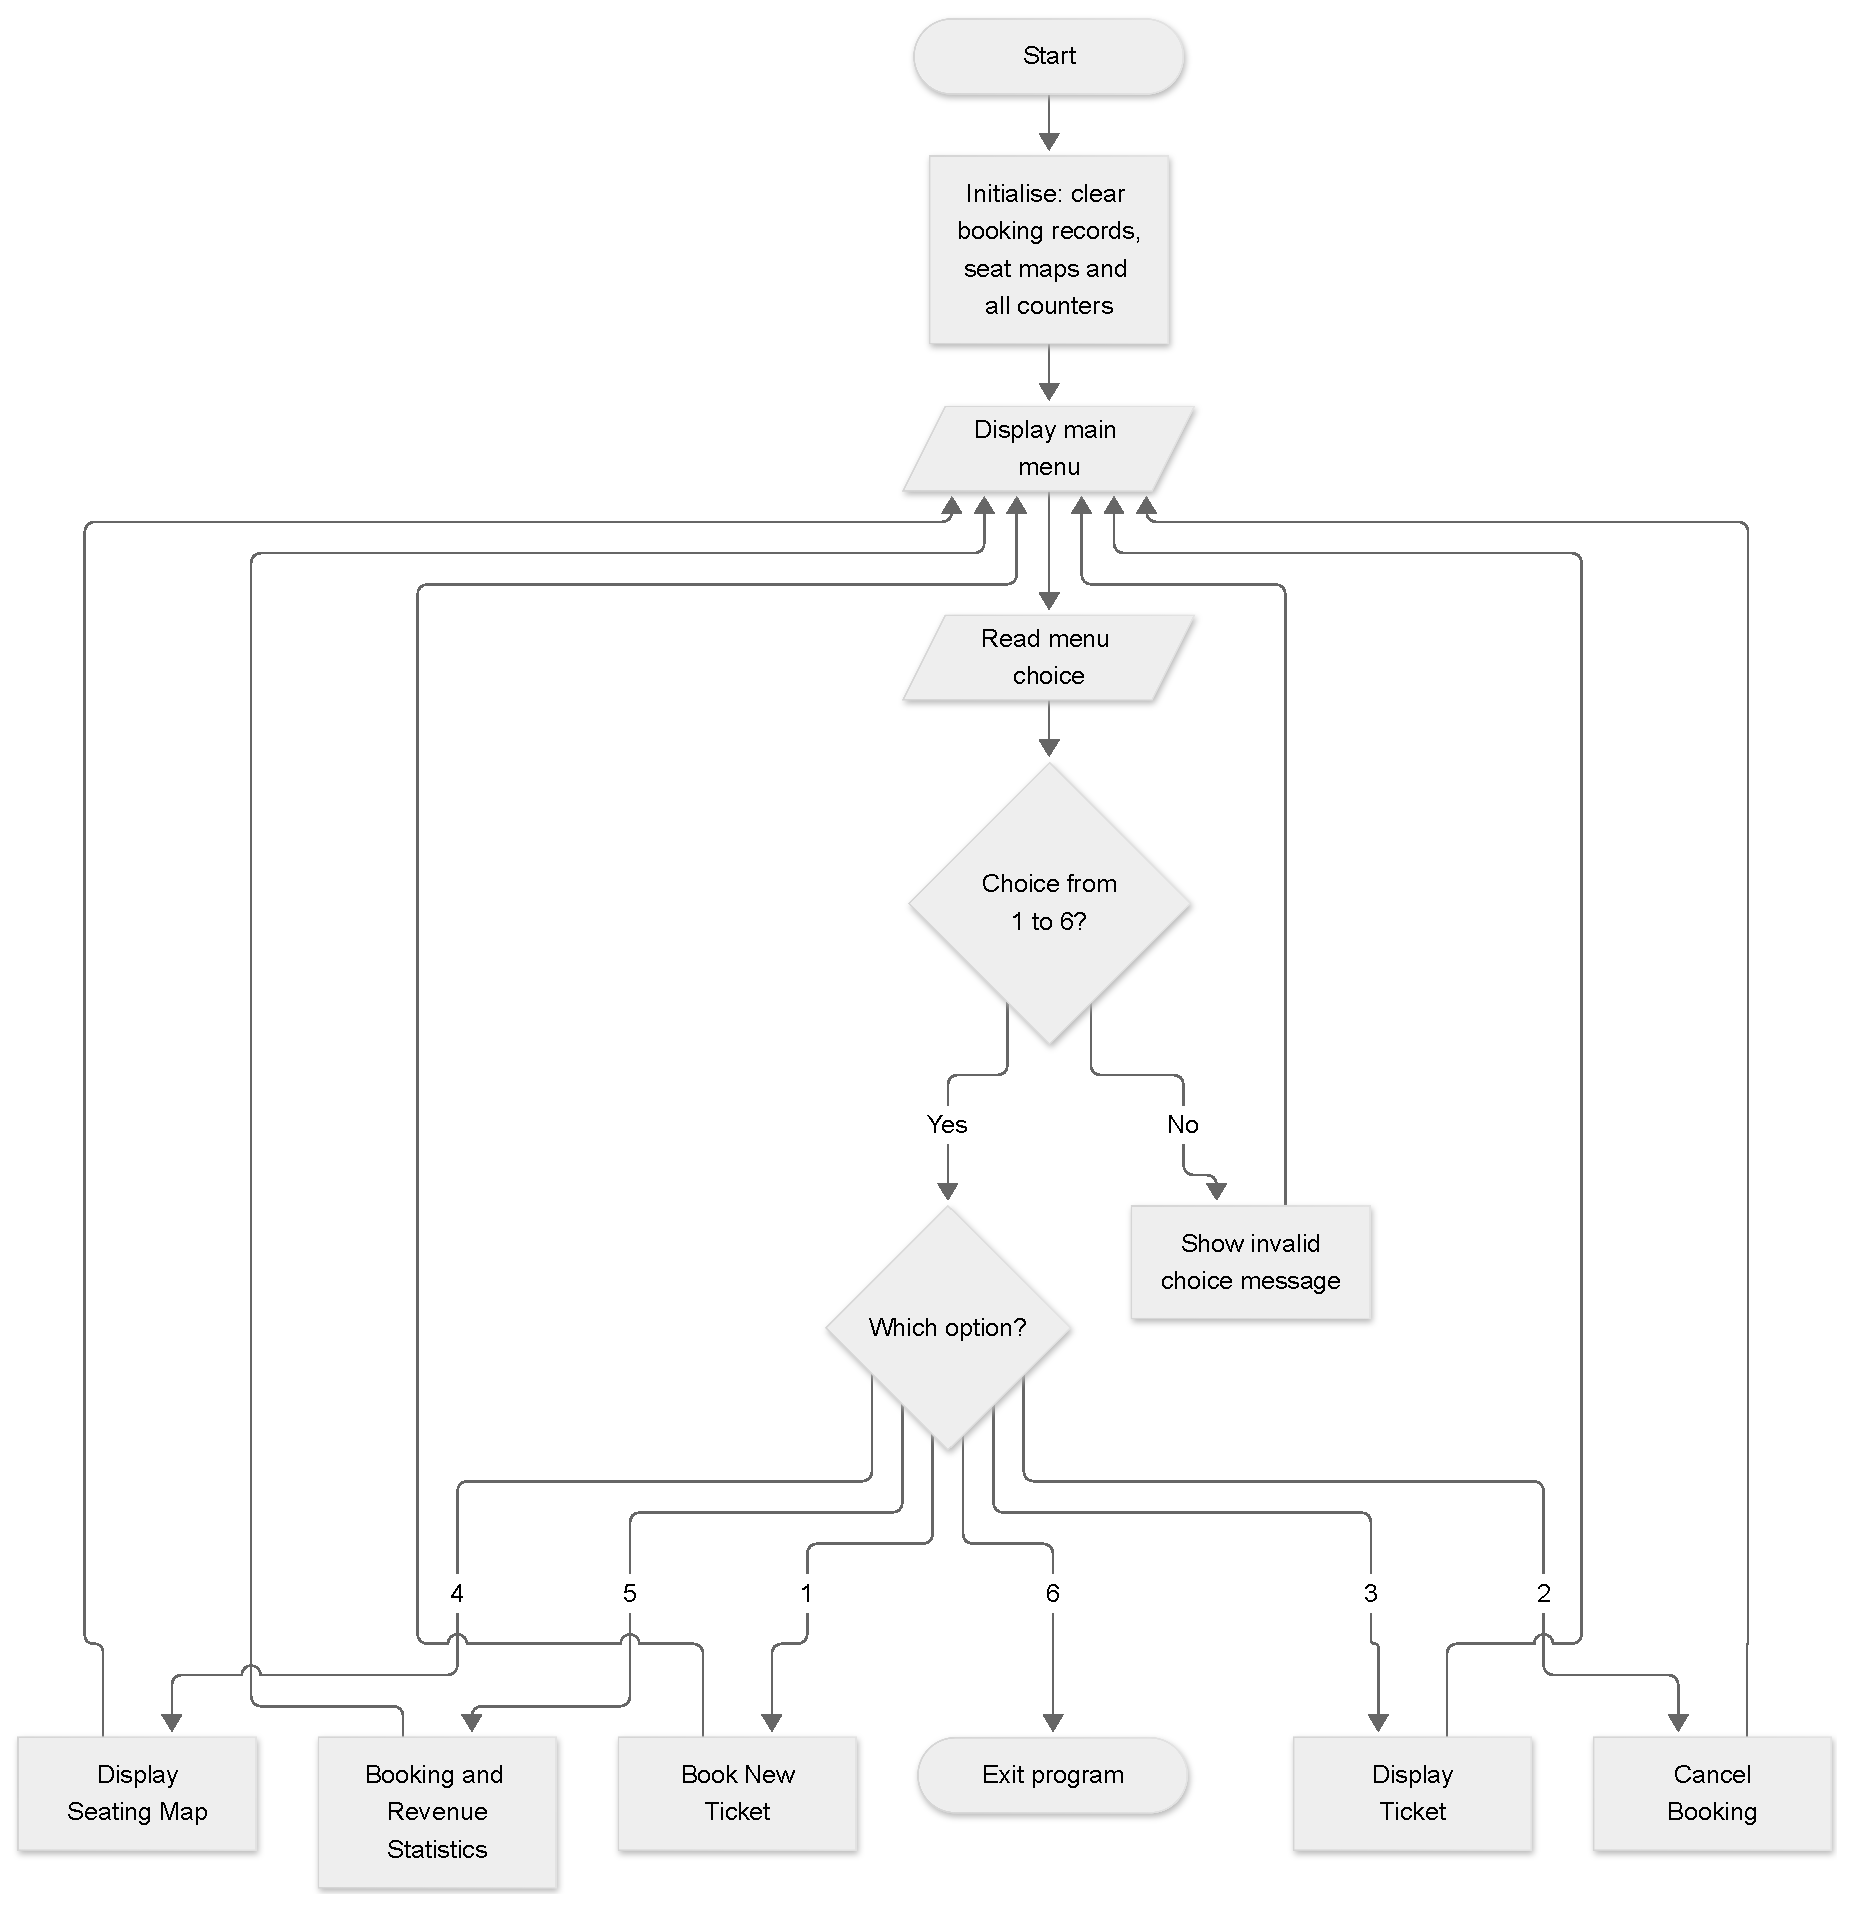
\includegraphics[width=0.85\textwidth]{diagrams/main-flow.pdf}
\captionof{figure}{Main program flow: menu loop and dispatch to the six operations.}
\label{fig:main-flow}
\end{minipage}

\medskip
Options 3 and 4 are short read-only operations. \textbf{Display Ticket} reads a booking ID, searches the records for an active match, and either prints the formatted ticket or reports \texttt{"ERROR: Booking ID not found!"}. \textbf{Display Seating Map} reads a movie code and prints that movie's 20 seats, each as \texttt{[O]} or \texttt{[X]}, followed by the reserved count and the occupancy percentage.

\subsection{Book New Ticket}

\begin{minipage}{\textwidth}
Each field is validated as soon as it is entered, so an invalid value is rejected immediately and re-read rather than being carried forward. The flow is shown in three parts (Figures~\ref{fig:book-a}--\ref{fig:book-c}): identity fields, seat selection, and pricing/commit.

\medskip
\centering
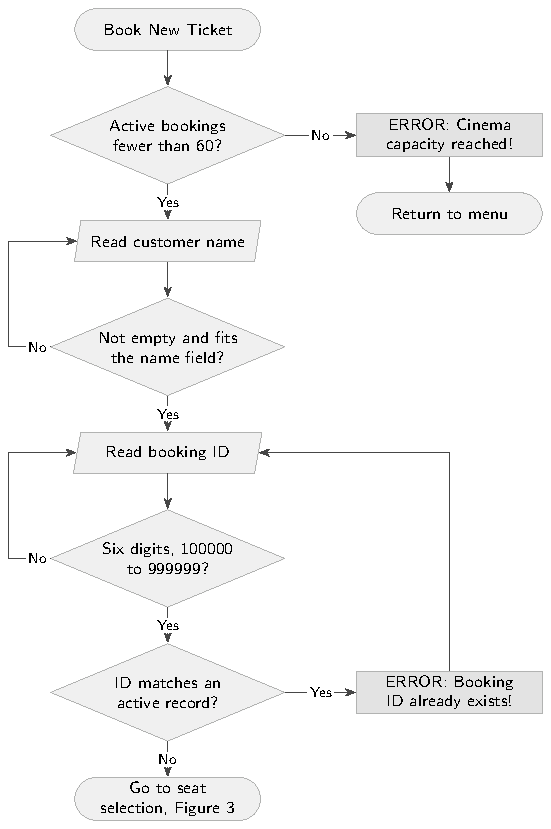
\includegraphics[height=0.68\textheight,width=0.95\textwidth,keepaspectratio]{diagrams/book-ticket-a.pdf}
\captionof{figure}{Book New Ticket, part 1: customer name and booking ID.}
\label{fig:book-a}
\end{minipage}

\begin{figure}[H]
\centering
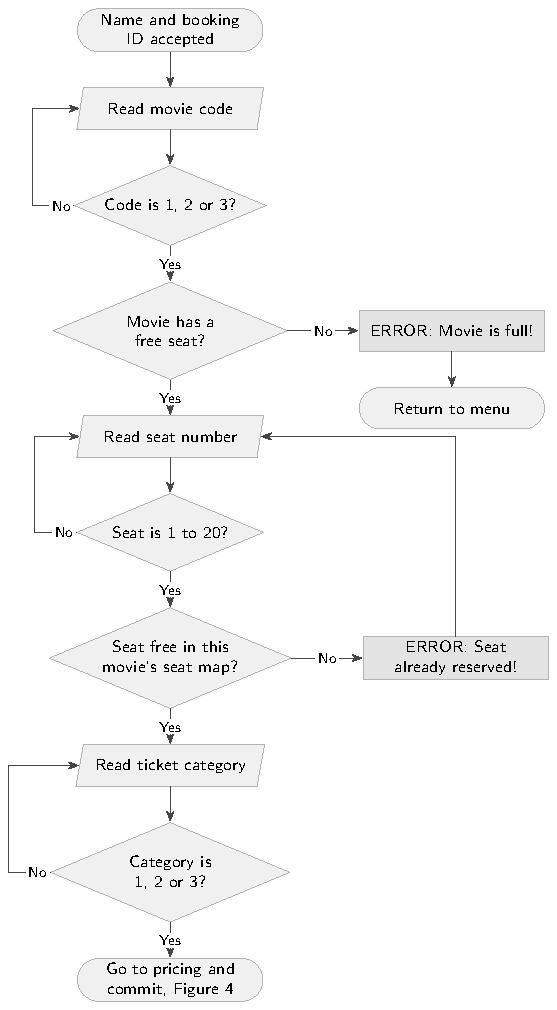
\includegraphics[height=0.72\textheight,width=0.95\textwidth,keepaspectratio]{diagrams/book-ticket-b.pdf}
\caption{Book New Ticket, part 2: movie code, seat number, ticket category.}
\label{fig:book-b}
\end{figure}

\begin{figure}[H]
\centering
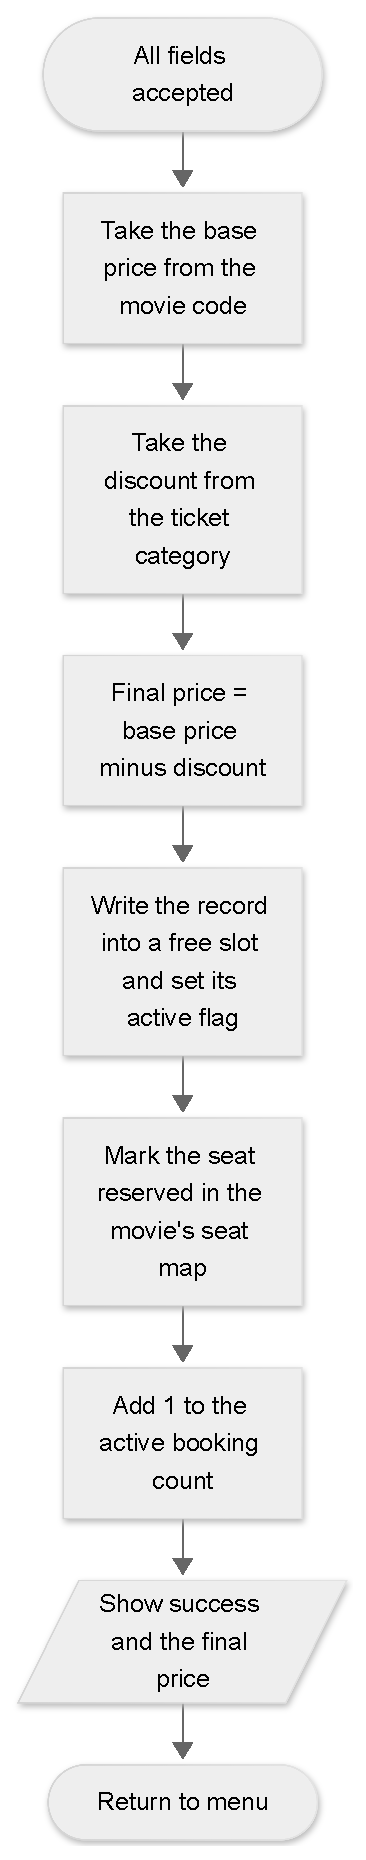
\includegraphics[height=0.72\textheight,width=0.95\textwidth,keepaspectratio]{diagrams/book-ticket-c.pdf}
\caption{Book New Ticket, part 3: pricing and commit to the booking record.}
\label{fig:book-c}
\end{figure}

\subsection{Cancel Booking}

\begin{minipage}{\textwidth}
Cancelling never deletes a record. It clears the record's active flag and releases the seat, which is what allows the same seat to be sold again in the same run.

\medskip
\centering
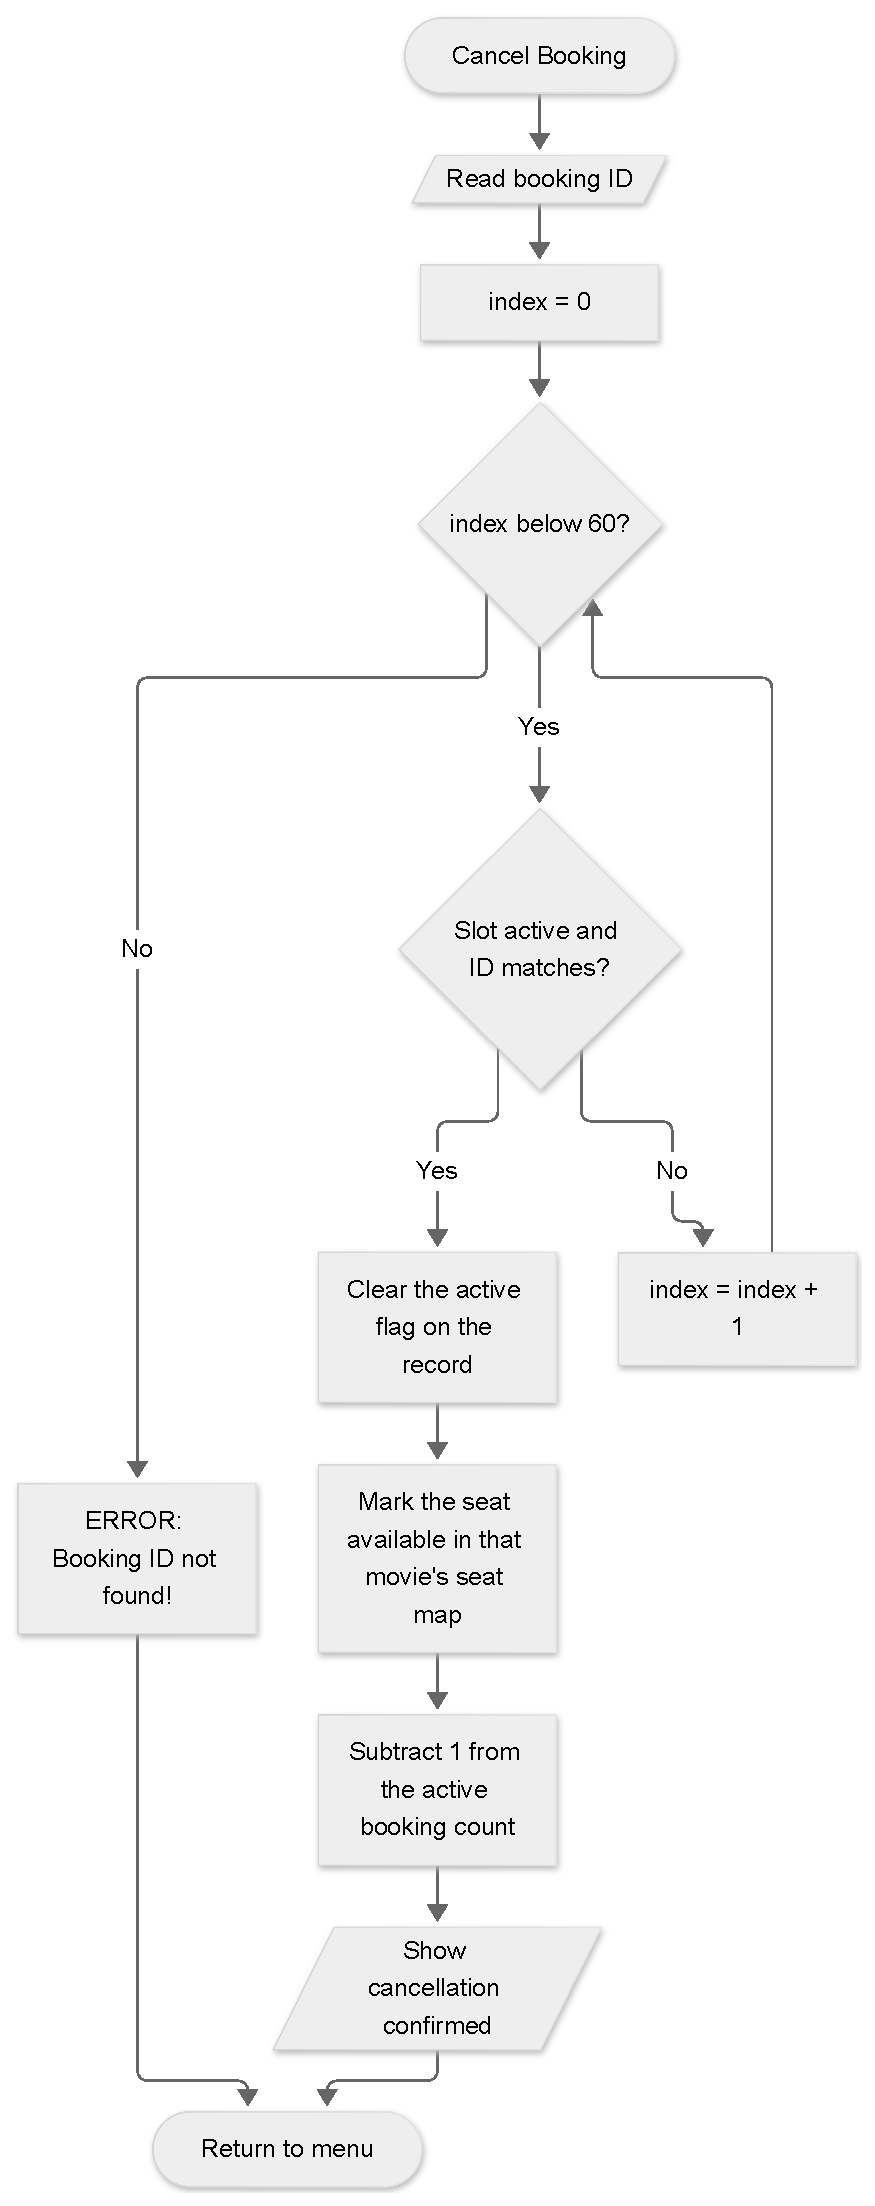
\includegraphics[height=0.68\textheight,width=0.95\textwidth,keepaspectratio]{diagrams/cancel-booking.pdf}
\captionof{figure}{Cancel Booking: linear search over 60 slots, then clear the active flag and free the seat.}
\label{fig:cancel}
\end{minipage}

\subsection{Booking and Revenue Statistics}

\begin{minipage}{\textwidth}
Every figure in the report is recalculated from the records at the moment the option is chosen, so the report is always current and inactive records never contribute to it. The flow is shown in two parts: the scan over all 60 slots (Figure~\ref{fig:stats-a}), and the derived figures and report (Figure~\ref{fig:stats-b}).

\medskip
\centering
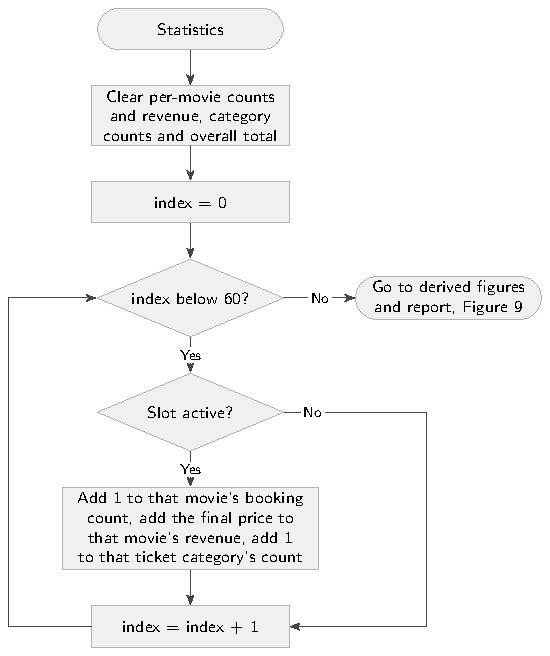
\includegraphics[height=0.62\textheight,width=0.95\textwidth,keepaspectratio]{diagrams/statistics-a.pdf}
\captionof{figure}{Statistics, part 1: scan the 60 record slots and accumulate per-movie and per-category counts.}
\label{fig:stats-a}
\end{minipage}

\begin{figure}[H]
\centering
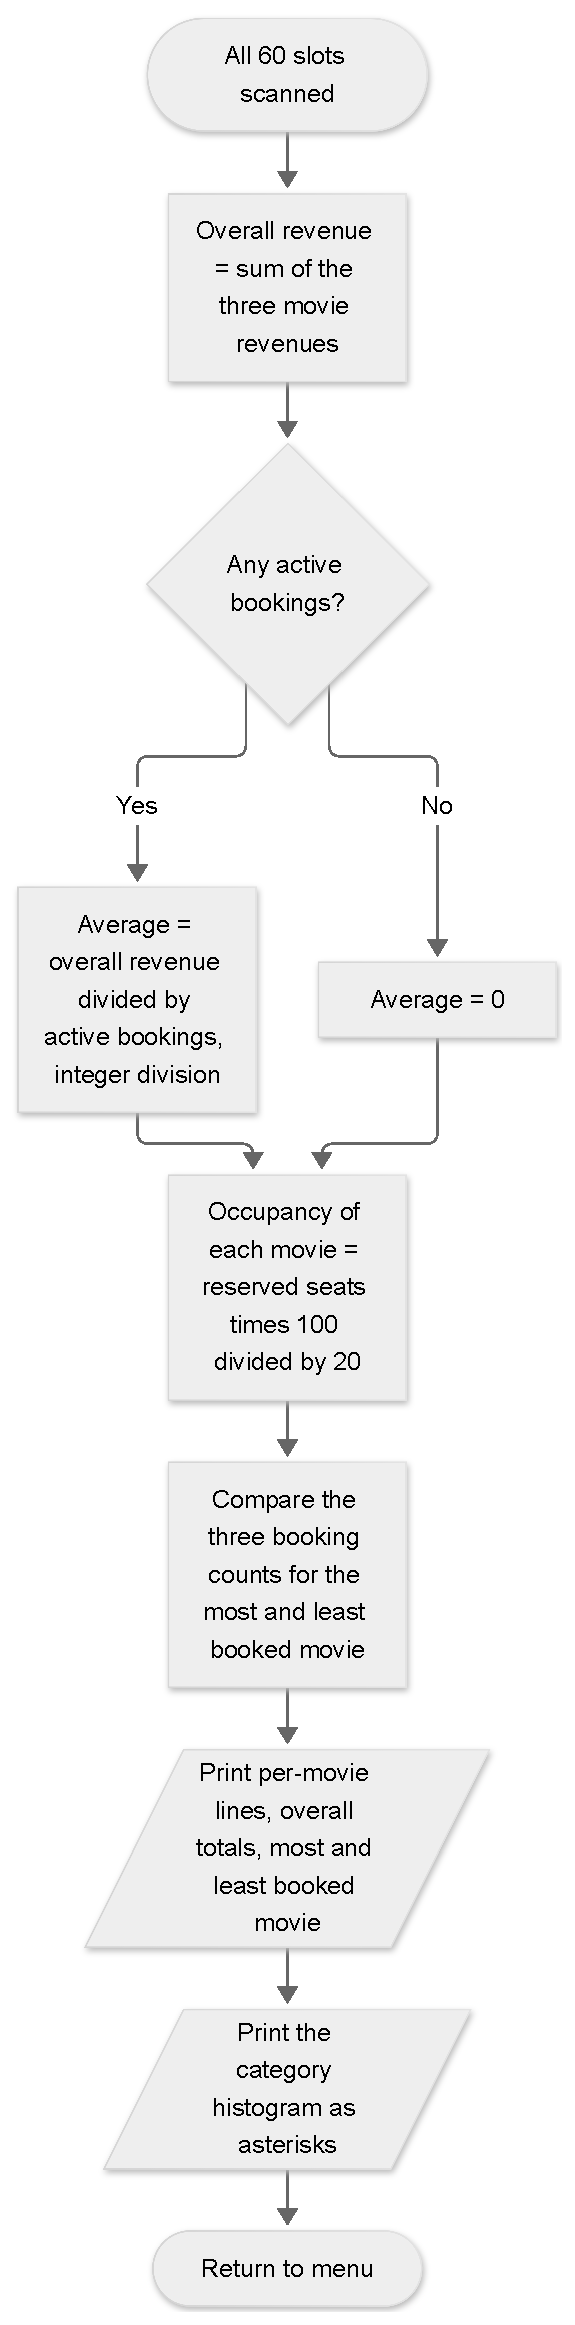
\includegraphics[height=0.72\textheight,width=0.95\textwidth,keepaspectratio]{diagrams/statistics-b.pdf}
\caption{Statistics, part 2: derive overall totals, average, occupancy, and print the report.}
\label{fig:stats-b}
\end{figure}

\subsection{Note on the repeated structures}

Three of the four flows above repeat an action a known number of times over a fixed array: the duplicate-ID check and the record scan both sweep 60 record slots, and the seating map prints 20 seats. Chapter Two identified CX as the processor's dedicated counter register, used by default for counted repetition, so the problem's shape fits that register naturally. The validation branches are different in kind: each one repeats \textit{until} the user supplies an acceptable value, so the number of repetitions is not known in advance. The project therefore requires both a counted repetition and a condition-controlled repetition, which satisfies the requirement for at least two loop structures.

\section{Constraints}

\subsection{Memory}

All storage is fixed in size and known before the program runs. Nothing is allocated while the program is running.

Each booking is stored as one fixed-size \textbf{record}: a single run of bytes holding every field for one ticket (name, ID, movie, seat, category, active flag, prices). The 60 records sit one after another in a fixed array, so a given booking is always found at the same offset: record index times record size. Table~\ref{tab:memory} breaks that record, and the system's other arrays, down byte by byte.

\begin{table}[H]
\centering
\caption{Memory used by the main data structures.}
\label{tab:memory}
\begin{tabular}{|l|l|l|}
\hline
\textbf{Structure} & \textbf{Size calculation} & \textbf{Total} \\
\hline
Booking records & 60 records, 37 bytes each & 2,220 bytes \\
\hline
Seat maps & 3 movies, 20 seats, 1 byte per seat & 60 bytes \\
\hline
Per-movie booking counts & 3 doublewords & 12 bytes \\
\hline
Per-movie revenue totals & 3 doublewords & 12 bytes \\
\hline
Ticket category counts & 3 doublewords & 12 bytes \\
\hline
\textbf{Total main data} & & \textbf{about 2.3 KB} \\
\hline
\end{tabular}
\end{table}

The 37-byte record is made up of a 21-byte name field (20 characters plus a null terminator), a 4-byte booking ID, three single bytes for movie code, seat number and category, one byte for the active flag, and two doublewords for the base price and final price.

\subsection{Registers against memory}

Chapter Two established that a processor has only a small, fixed set of registers, that they are fast but temporary, and that program data lives in main memory. CTRMS holds roughly 2.3 KB of state, so the records, the seat maps and the counters must all live in memory. Registers can only ever hold what is being worked on at that instant: the current array index, a loop counter, an address, or the result of one arithmetic step. This is the reason the system is built around arrays indexed by position rather than around values kept permanently in registers.

\subsection{Capacity}

\begin{itemize}
\item At most \textbf{60 active bookings} at any one time.
\item Exactly \textbf{3 movies}, fixed, not configurable.
\item Exactly \textbf{20 seats} per movie, so at most 60 seats in total across the cinema.
\item Customer names limited to \textbf{20 characters}, stored in a 21-byte field with the null terminator.
\item Booking IDs limited to the \textbf{900,000 values} from 100000 to 999999.
\end{itemize}

\subsection{Integer arithmetic}

The processor does provide floating-point registers, as covered in Chapter Two, but the project specification forbids floating-point instructions. Every calculation is therefore integer arithmetic, with these consequences:

\begin{itemize}
\item \textbf{Prices are exact.} Base prices are 8, 7 and 6 JOD and discounts are 0, 1 and 2 JOD, so every final price is a whole number from 4 to 8 JOD. No rounding occurs.
\item \textbf{Occupancy is exact.} Occupancy is \textit{reserved seats times 100 divided by 20}, which is the same as \textit{reserved seats times 5}. Every value from 0 to 20 seats therefore maps to an exact percentage from 0 to 100, and nothing is lost to truncation.
\item \textbf{The average ticket price is the only figure that loses precision.} It is \textit{overall revenue divided by active bookings} in integer division, so the remainder is discarded. For example, 26 JOD over 4 bookings gives 6 JOD, not 6.5 JOD. The report shows the truncated value, which is what the specification requires.
\end{itemize}

\subsection{Value ranges}

Three range limits act as hard constraints on the design:

\begin{enumerate}
\item A booking ID can reach 999,999, which exceeds the 65,535 limit of a word, so IDs must occupy a doubleword.
\item Movie codes, seat numbers, categories and the active flag all stay within 0 to 255 and therefore fit in a single byte each.
\item The largest revenue the system can ever hold is 60 bookings at the top price of 8 JOD, which is \textbf{480 JOD}. This is nowhere near the doubleword limit, so no overflow handling is needed for any total.
\end{enumerate}

Every quantity in the system (identifiers, counts, prices, revenue, percentages) is non-negative. All values are therefore treated as unsigned, and the two's-complement representation of negative numbers studied in Chapter One does not arise anywhere in this project.

\subsection{Platform and course constraints}

\begin{itemize}
\item The program is written in x86 assembly for \textbf{MASM with the Irvine32 library}, and runs as a 32-bit Windows console application in \textbf{protected mode}, the native mode described in Chapter Two.
\item There is \textbf{no persistence}. All records live in memory only, so every booking is lost when the program exits.
\item The program is \textbf{console only}. There is no graphical interface, no mouse input and no printing.
\item The course imposes its own requirements that shape the design: at least \textbf{8 procedures}, at least \textbf{2 different loop structures}, IF, IF-ELSE and nested conditionals, and the use of all five required data types: strings, doublewords, bytes, characters and arrays.
\end{itemize}

\section{Assumptions}

\begin{enumerate}
\item \textbf{Seats belong to a movie, not to the cinema.} Seat 5 of Movie A and seat 5 of Movie B are different seats. A seat is unavailable only when that same movie and seat number are already reserved.
\item \textbf{Cancelled records stay in the array.} Cancelling clears the active flag; it does not erase the record or shift any other record. Only the active flag decides whether a record counts.
\item \textbf{Inactive records are invisible to every report.} They are excluded from the active booking count, from all revenue, from occupancy and from the category histogram.
\item \textbf{A freed slot and a freed seat are both reusable.} After a cancellation the record slot can hold a new booking and the seat can be sold again in the same run.
\item \textbf{A booking ID is unique among active bookings only.} Once a booking is cancelled, its ID may be used again by a new booking.
\item \textbf{One booking is one seat, one ticket and one customer.} There is no group booking and no multi-seat purchase in a single transaction.
\item \textbf{One user at a time.} The program is a single console session with no concurrent access, so no two bookings can ever be made at the same instant.
\item \textbf{Prices are fixed constants.} The three base prices and the three discounts are built into the program and are never entered or changed at runtime.
\item \textbf{All input arrives as ASCII text from the keyboard.} Where a number is expected, anything that is not a valid number in range is treated as invalid input and the prompt is repeated.
\item \textbf{The user is cinema staff, not the public.} The person at the keyboard is assumed to be trained in the menu, so prompts explain the legal range but no further help system is provided.
\item \textbf{All lab machines behave identically.} Every machine runs the same MASM and Irvine32 setup in protected mode, so no machine-specific behaviour is relied upon.
\end{enumerate}

\clearpage

% ---------- Change header and numbering for Chapter Three ----------
\fancyhead[C]{\bfseries Chapter Three: Requirements Specification}
\renewcommand{\thesection}{3.\arabic{section}}
\renewcommand{\thesubsection}{3.\arabic{section}.\arabic{subsection}}
\setcounter{section}{0}

% ---------- Chapter-opening page ----------
\thispagestyle{empty}
\vspace*{\stretch{1}}
\begin{center}
{\Large\bfseries Chapter Three}\\[1em]
{\Large\bfseries Requirements Specification}
\end{center}
\vspace*{\stretch{2}}
\clearpage

\section{Functional Requirements}

The system must fulfill the following functional requirements to meet the project objectives. Priorities are classified as High (H), Medium (M), or Low (L).

\begin{table}[H]
\centering
\caption{Functional Requirements}
\label{tab:func-req}
\renewcommand{\arraystretch}{1.3}
\begin{tabular}{|p{0.1\linewidth}|p{0.75\linewidth}|p{0.05\linewidth}|}
\hline
\textbf{ID} & \textbf{Description} & \textbf{Pri} \\
\hline
FR01 & The system shall display a main menu with six options: Book, Cancel, Display Ticket, Display Seating Map, Statistics, and Exit.& H \\
\hline
FR02 & The system shall record new ticket bookings by accepting Customer Name, Booking ID, Movie Code, Seat Number, and Ticket Category. & H \\
\hline
FR03 & The system shall validate that the 6-digit Booking ID is unique and falls between 100000 and 999999. & H \\
\hline
FR04 & The system shall calculate final ticket prices by subtracting the applicable ticket category discount from the movie's base price. & H \\
\hline
FR05 & The system shall prevent duplicate seat reservations for the same movie hall. & H \\
\hline
FR06 & The system shall deactivate a booking and release its seat when a user cancels an active booking using its ID. & H \\
\hline
FR07 & The system shall format and display an individual ticket, including all pricing and discount details, when provided a valid active Booking ID. & M \\
\hline
FR08 & The system shall output a visual seating map for a specified movie, indicating available seats with \texttt{[O]} and reserved seats with \texttt{[X]}. & M \\
\hline
FR09 & The system shall calculate and display revenue statistics, total bookings, occupancy percentages, and a ticket category distribution histogram. & M \\
\hline
FR10 & The system shall restrict total active bookings to a maximum capacity of 60 reservations across the three movies. & H \\
\hline
\end{tabular}
\end{table}

\section{Non-Functional Requirements}

The following constraints define the technical environment, structural quality, and architectural standards of the system.

\begin{table}[H]
\centering
\caption{Non-Functional Requirements}
\label{tab:non-func-req}
\renewcommand{\arraystretch}{1.3}
\begin{tabular}{|p{0.09\linewidth}|p{0.82\linewidth}|}
\hline
\textbf{ID} & \textbf{Description} \\
\hline
NFR01 & The software shall be implemented entirely in x86 Assembly Language using MASM. \\
\hline
NFR02 & The software shall utilize the Irvine32 library for all console input/output and string formatting operations. \\
\hline
NFR03 & The software shall rely exclusively on integer arithmetic for all pricing and statistical calculations; floating-point instructions are strictly forbidden. \\
\hline
NFR04 & The software shall use fixed-size memory records and arrays to manage the state of the up to 60 active booking entries. \\
\hline
\end{tabular}
\end{table}

\section{CLO Mapping}

The specified requirements directly support the Course Learning Outcomes (CLOs) as defined in the project structure:

\begin{itemize}
    \item \textbf{S1: Develop assembly language programs for microcomputers to perform basic input/output operations.}
    \begin{itemize}
        \item \textbf{Mapping:} Supported by FR01, FR07, FR08, and FR09. The system fulfills this outcome by prompting the user for input, executing validation loops, and rendering highly formatted reports (menus, tickets, seating maps, and histograms) directly to the console[cite: 13].
    \end{itemize}
    
    \item \textbf{S2: Implement and debug assembly language programs that perform arithmetic, string operations, searching, and memory manipulation tasks.}
    \begin{itemize}
        \item \textbf{Mapping:} Supported by FR02, FR04, FR06, and NFR04. The logic explicitly requires iterating over arrays to perform searches (booking IDs, seat availability), reading strings (customer names), and executing integer arithmetic to calculate ticket pricing and cumulative statistics.
    \end{itemize}

    \item \textbf{C1: Distinguish between different processor registers and use them appropriately in assembly language programming.}
    \begin{itemize}
        \item \textbf{Mapping:} Supported by NFR01 and NFR03. The implementation mandates correct assignment and management of general-purpose registers (EAX, EBX, ECX, EDX, ESI, EDI) according to standard architectural conventions for calculations, pointers, loop counting, and library parameter passing.
    \end{itemize}
\end{itemize}

\end{document}